\documentclass[a4paper, 12pt, twoside]{article}
\usepackage{mathptmx} % approximate Times New Roman
\usepackage{graphicx} %graph
\usepackage{subcaption}
\usepackage[doublespacing]{setspace}
\usepackage{geometry} %setting margin
\usepackage{array}
\usepackage{url}
\geometry{top=2.5cm, bottom=2.5cm, outer = 2.5cm, inner=4cm}
\usepackage{lipsum} %having the example content to fill the part
\usepackage[utf8]{inputenc}
\usepackage{amsmath} %formular
\usepackage{booktabs} % for the tables
\usepackage{longtable,lscape}
\usepackage{rotating}
\usepackage{multirow,multicol}
\usepackage{mathtools}
\usepackage{IEEEtrantools}
\usepackage{rotating}
%\usepackage[breaklinks]{hyperref}
%\usepackage{apacite}
\usepackage[flushleft]{threeparttable}
\usepackage{listings}
\usepackage{apacite}
\bibliographystyle{apacite}
%\usepackage{natbib}
\usepackage{csquotes}
\usepackage{sectsty} %set the font for sections
\allsectionsfont{\normalsize \bf}
\sectionfont{\centering \bf \normalsize}
\usepackage[titletoc]{appendix}
\usepackage[none]{hyphenat}
\usepackage{threeparttable}
\usepackage{afterpage}
\newcommand{\pkg}[1]{{\normalfont\fontseries{b}\selectfont #1}}
\let\proglang=\textsf
\let\code=\texttt
\usepackage{color}
\usepackage{caption}
\newcolumntype{L}[1]{>{\raggedright\let\newline\\\arraybackslash\hspace{0pt}}m{#1}}
\newcolumntype{C}[1]{>{\centering\let\newline\\\arraybackslash\hspace{0pt}}m{#1}}
\newcolumntype{R}[1]{>{\raggedleft\let\newline\\\arraybackslash\hspace{0pt}}m{#1}}

%\usepackage{titletoc}
%\newcolumntype{P}[1]{>{\raggedright}p{#1\linewidth}}

%set the table of contents

\usepackage{tocstyle}
\usetocstyle{standard}
\settocfeature{raggedhook}{\raggedright}

\definecolor{asparagus}{rgb}{0.53, 0.66, 0.42}
\definecolor{gray}{rgb}{0.5,0.5,0.5}
\definecolor{mauve}{rgb}{0.58,0,0.82}
\definecolor{antiquefuchsia}{rgb}{0.57, 0.36, 0.51}
\definecolor{ao(english)}{rgb}{0.0, 0.5, 0.0}
\definecolor{armygreen}{rgb}{0.29, 0.33, 0.13}
\definecolor{ao}{rgb}{0.0, 0.0, 1.0}
\definecolor{bananayellow}{rgb}{1.0, 0.88, 0.21}

\lstset{frame=tb,
	language=R,
	basicstyle=\small \ttfamily, % the size of the fonts that are used for the code
	numbers=left,                   % where to put the line-numbers
	numberstyle=\tiny\color{Blue},  % the style that is used for the line-numbers
	stepnumber=1,
	aboveskip=3mm,
	belowskip=3mm,
	showstringspaces=false,
	columns=flexible,
	numbers=none,
	keywordstyle=\color{ao(english)},
	numberstyle=\tiny\color{gray},
	commentstyle=\color{ao},
	stringstyle=\color{mauve},
	breaklines=true,                % sets automatic line breaking
	breakatwhitespace=false,        % sets if automatic breaks should only happen at whitespace
	tabsize=3
}
 %-=======Table and figure format
 \DeclareCaptionLabelSeparator*{spaced}{\\[2ex]}
 \captionsetup[table]{textfont=it,format=plain,justification=justified,
 	singlelinecheck=false,labelsep=spaced,skip=0pt}
 \captionsetup[figure]{labelsep=period,labelfont=it,justification=justified,
 	singlelinecheck=false,font=doublespacing}

%% From "Latex Companion": Spaces between words:
\tolerance=2000
\emergencystretch=20pt
\begin{document}

%----------------------------Thesis Cover----------------------------%
\newgeometry{top=5.3cm, bottom=2.54cm, outer = 2.54cm, inner=2.54cm}
\begin{titlepage}
	\begin{center}
	\doublespacing
	Thesis Title\\ %% if it is too long you could use \\ after each line
	[1.5cm]
	by\\
	[1.5cm]
	Name of Author\\
	[2.4cm]
	Doctor of Philosophy in Psychology\\
	[4.5cm]
	2020\\
	[1cm]
		\begin{figure}[h]
			\centering
			
\includegraphics[width = 31mm]{fig/umac_logo}
		\end{figure}
	Faculty of Social Sciences\\
	University of Macau
	\end{center}
\end{titlepage}
%----------------------------Title Page----------------------------%
\begin{titlepage}
	\begin{center}
	\doublespacing
	Thesis Title \\%% if it is too long you could use \\ after each line
	[1.8cm]
	by\\
	[1.8cm]
	Name of Author\\
	[1.8cm]
	SUPERVISOR: Name of Supervisor\\
	[1.8cm]
	DEPARTMENT: Name of Department\\
	[1.8cm]
	Degree Title\\
	[1.8cm]
	2020\\
	[1.8cm]
	University of Macau
	\end{center}
\end{titlepage}
%----------------------------Author's Right----------------------------%
\begin{titlepage}
\newgeometry{top = 10cm}
\begin{center}
Author's right 2020 by\\
SURNAME, Given Names
\end{center}
\end{titlepage}
\newpage\null\thispagestyle{empty}\newpage

\restoregeometry
\setcounter{page}{1}
\pagenumbering{roman}
%----------------------------Acknowledgements----------------------------%
\section*{Acknowledgements}
\addcontentsline{toc}{section}{\numberline{}Acknowledgements}
Here you could put the persons you want to thanks. 

\newpage

%----------------------------Abstract---------------------------%
\section*{Abstract}
\addcontentsline{toc}{section}{\numberline{}Abstract}
The title Abstract should be in bold and centered. The abstract must not be more than 350 words
\newpage

%----------------------------Declaration----------------------------%
\section*{Declaration}
\addcontentsline{toc}{section}{\numberline{}Declaration}
%This is the English version of Declaration
I declare that the thesis here submitted is original except for the source materials explicitly acknowledged  and that this thesis as a whole, or any part of this thesis has not been previously submitted for the same degree or for a different degree.\\ \\ 
I also acknowledge that I have read and understood the Rules on Handling Student Academic Dishonesty and the Regulations of the Student Discipline of the University of Macau.

\newpage
%----------------------------Table of Contents----------------------------

\renewcommand\contentsname{Table of Contents}
\tableofcontents

\newpage
\singlespacing
\listoffigures
\newpage
\listoftables

%----------------------------CH1 Introduction----------------------------%
\newpage 
\setcounter{page}{1}
\pagenumbering{arabic}
\section*{Chapter 1 Introduction}
\addcontentsline{toc}{section}{\numberline{}Chapter 1 Introduction}
\label{sec:intro}
\setcounter{section}{1}
\doublespacing
You can write the first chapter here. 

The APA style citing: for example, you mentioned something \cite{abelson1985variance}. Or \citeA{abelson1985variance} mentioned something very important. 

Below is two subsections which the Graduate School asked me to put. 

\subsection{Potential Contributions}
You can write something here.

\subsection{Statement of Originality}
You can write something here. 

%----------------------------CH2 Literature Review----------------------------%
\newpage
\section*{Chapter 2 Literature Review}
\addcontentsline{toc}{section}{\numberline{}Chapter 2 Literature Review}
\label{sec:lr}
\setcounter{section}{2}
\setcounter{subsection}{0}
\doublespacing
How to quote: 

\begin{quote}
	Without intending any necessary implication of causality, it is convenient to use the phrase “effect size” to mean “the degree to which the phenomenon is present in the population,” or “the degree to which the null hypothesis is false.”. By the above route it can now readily be clear that when the null hypothesis is false, it is false to some specific degree, i.e., the effect size (ES) is some specific non-zero value in the population. The larger this value, the greater the degree to which the phenomenon under study is manifested. (pp. 9-10)
\end{quote}
 If you quote, you have to quote in this way: ``a named expression that maps data, statistics, or parameters onto a quantity that represents the magnitude of some phenomenon" \cite[p.141]{kelley2012effect}. 
 
Examples of Equations:
\begin{equation}
\delta = \frac{\mu^E - \mu^C}{\sigma},
\label{pop_smd}
\end{equation}
 


%----------------------------Reference----------------------------%
\newpage
\singlespacing
\raggedright
\bibliography{ref}


%--------------------------Tables---------------------------%
%Chapter 1--------------------%
	\begin{landscape}
	\singlespacing
	%\begin{center}
	\begin{longtable}[l]{cL{4cm} R{1.5cm}  R{1.5cm} R{1.5cm}R{1.5cm}  R{1.5cm}  R{1.5cm} R{1.5cm}R{1.5cm} R{1.5cm}R{1.5cm}}
		\caption{Characteristics of the Meta-Analysis Conducted by Bora et al. (2009) } 	\label{tab:ex_ToM} \\		
		
		\hline
		No & Study & 
		$n_1$ & $m_1$ & $sd_1$ & $CV_1$ & 
		$n_2$ & $m_2$ & $sd_2$ & $CV_2$ & P. Max & $d$ \\
		\hline 
		\endfirsthead
		
		\multicolumn{12}{c}%
		{{\bfseries \tablename\ \thetable{} -- continued from previous page}} \\
		\hline 
		No & Study & 
		$n_1$ & $m_1$ & $sd_1$ & $CV_1$ & 
		$n_2$ & $m_2$ & $sd_2$ & $CV_2$ & P. Max & $d$ \\
		\hline 
		\endhead
		
		\multicolumn{12}{r}{{Continued on next page}} \\ \hline
		\endfoot
		
		\hline 
		\endlastfoot
		
		1 & Corcoran et al., 1995 \nocitemeta{corcoran1995schizophrenia}
		& 55 & 15.60 & 3.90 & 25.00 & 30 & 18.30 & 1.60 & \textbf{8.74} & 20 & 0.822 \\       
		2 & Sarfati et al., 1997 \nocitemeta{sarfati1997attribution}
		& 24 & 18.40 & 6.70 & 36.41 & 24 & 24.90 & 2.10 & \textbf{8.43} & 28 & 1.309\\        
		3 & Sarfati et al., 1999a \nocitemeta{sarfati1999how}
		& 25 & 9.90 & 3.69 & 37.27 & 15 & 13.20 & 0.90 & \textbf{6.82} & 14 & 1.106\\       
		4 & Sarfati et al., 1999b \nocitemeta{sarfati1999investigating}
		& 26 & 18.65 & 6.45 & 34.56 & 13 & 24.40 & 2.30 & \textbf{9.43} & 28 & 1.053\\
		5 & Russell et al., 2000 \nocitemeta{russell2000exploring} 
		& 5 & 12.60 & 5.03 & 39.92 & 7 & 6.16 & 3.84 & 62.34 & 30 & 1.479 \\       
		6 & Kington et al., 2000 \nocitemeta{kington2000impaired}
		& 16 & 7.75 & 1.24 & 16.00 & 16 & 9.06 & 0.85 & \textbf{9.38} & 10 & 1.232 \\      
		7 & Langdon et al., 2001 \nocitemeta{langdon2001visual}
		& 32 & 4.05 & 1.38 & 34.07 & 24 & 5.50 & 0.78 & \textbf{14.18} & 6 & 1.247\\       
		8 & Langdon et al., 2002 \nocitemeta{langdon2002disturbed}
		& 25 & 3.79 & 1.36 & 35.88 & 20 & 5.54 & 0.76 & \textbf{13.72} & 6 & 1.542\\       
		9 & Langdon et al., 2002 \nocitemeta{langdon2006externalizing}
		& 25 & 0.66 & 0.25 & 37.88 & 20 & 0.92 & 0.12 & \textbf{13.04} & 1 &1.280 \\      
		10& Brunet et al., 2003 \nocitemeta{brunet2003reasoning}
		& 25 & 11.10 & 2.80 & 25.23 & 25 & 13.00 & 1.20 & \textbf{9.23} & 14 & 0.882 \\    
		11 & Randall et al., 2003 \nocitemeta{randall2003attention}
		& 32 & 3.61 & 2.22 & 61.37 & 18 & 5.43 & 1.40 & 25.78 & 6 & 0.925 \\      
		12 & Randall et al., 2003 
		& 32 & 1.64 & 1.96 & \textbf{119.50} & 18 & 4.57 & 1.6 & 35.01 & 6 & 1.591\\      
		13 & Corcoran \& Frith 2003 \nocitemeta{corcoran2003autobiographical}
		& 59 & 2.42 & 1.04 & 42.98 & 44 & 3.65 & 0.49 & \textbf{13.42} & 4 & 1.446\\      
		14 & Corcoran \& Frith 2003 
		& 59 & 14.86 & 5.32 & 35.8 & 44 & 18.90 & 1.02 & \textbf{5.4} & 20 & 0.964\\    
		15 & Craig et al., 2004 \nocitemeta{craig2004persecutory}
		& 16 & 15.75 & 3.34 & 21.21 & 16 & 19.56 & 0.73 & \textbf{3.73} & 20 & 1.576\\     
		16 & Craig et al., 2004 
		& 16 & 18.19 & 6.65 & 36.56 & 16 & 27.63 & 4.43 & 16.03 & 36 & 1.671 \\     
		17 & Harrington et al., 2005a \nocitemeta{harrington2005schizophrenia}
		& 25 & 4.46 & 1.20 & 26.91 & 38 & 5.16 & 0.99 & 19.19 & 6 & 0.650\\  
		18 & Harrington et al., 2005a 
		& 25 & 76.70 & 22.90 & 29.86 & 38 & 87.20 & 16.00 & 18.35 & 100 & 0.552 \\ 
		19 & Harrington et al., 2005a 
		& 25 & 54.60 & 29.80 & 54.58 & 38 & 72.20 & 19.70 & 27.29 & 100 & 0.728\\
		20 & Marjoram et al., 2005 \nocitemeta{marjoram2005symptomatology}
		& 15 & 15.50 & 2.20 & \textbf{14.19} & 15 & 19.20 & 1.10 & \textbf{5.73} & 20 &2.127\\       
		21 & Br{\"u}ne \& Bodenstein 2005 \nocitemeta{brune2005proverb}
		& 31 & 25.30 & 8.40 & 33.20 & 21 & 35.30 & 1.30 & \textbf{3.68} & 36 & 1.525\\    
		22 & Br{\"u}ne \& Bodenstein 2005 
		& 31 & 40.80 & 12.00 & 29.41 & 21 & 56.30 & 2.90 & \textbf{5.15} & 59 & 1.636 \\    
		23 & Kelemen et al., 2005 \nocitemeta{kelemen2005theory}
		& 52 & 18.50 & 5.20 & 28.11 & 30 & 22.50 & 2.90 & \textbf{12.89} & 29 & 0.888 \\    
		24 & Langdon et al., 2006 \nocitemeta{langdon2006externalizing}
		& 34 & 3.74 & 1.60 & 42.69 & 21 & 5.60 & 0.56 & \textbf{10.00} & 6 & 1.429\\     
		25 & Pinkham \& Penn, 2006 \nocitemeta{pinkham2006neurocognitive}
		& 49 & 3.06 & 0.88 & 28.69 & 44 & 3.58 & 0.63 & 17.49 & 4 & 0.677 \\     
		26 & Pinkham \& Penn, 2006 
		& 49 & 15.10 & 4.06 & 26.91 & 44 & 17.14 & 2.12 & \textbf{12.38} & 20 & 0.620\\
		27 & Martino et al., 2007 \nocitemeta{martino2007neuropsychological}
		& 21 & 0.82 & 0.11 & \textbf{13.41} & 15 & 0.94 & 0.05 & \textbf{5.32} & 1 & 1.329\\     
		28 & Br{\"u}ne et al., 2007 \nocitemeta{brune2007mental}
		& 38 & 29.20 & 6.00 & 20.55 & 29 & 34.00 & 2.50 & \textbf{7.35} & 36 & 0.997\\                
		29 & Br{\"u}ne et al., 2007
		& 38 & 19.20 & 3.50 & 18.23 & 29 & 21.90 & 1.40 & \textbf{6.39} & 23 & 0.966\\       
		30 & Bertrand et al., 2007 \nocitemeta{bertrand2007social}
		& 36 & 15.31 & 3.11 & 20.31 & 27 & 18.07 & 1.47 & \textbf{8.14} & 20 & 1.085\\  
		31 & Pousa et al., 2008 \nocitemeta{pousa2008theory}
		& 61 & 4.06 & 1.55 & 38.18 & 51 & 4.20 & 1.14 & 27.14 & 6 & 0.102 \\       
		32 & Pousa et al., 2008 
		& 61 & 1.23 & 0.76 & 61.79 & 51 & 1.41 & 0.67 & 47.52 & 2  & 0.250\\       
		33 & B{\^a} et al., 2008 \nocitemeta{ba2008deficits}
		& 16 & 2.69 & 0.60 & 22.3 & 16 & 3.00 & 0 & \textbf{0} & 3 &0.731\\           
		34 & Mo et al., 2008 \nocitemeta{mo2008comprehension}
		& 29 & 1.17 & 0.71 & 60.68 & 22 & 1.95 & 0.21 & \textbf{10.77} & 2 & 1.375 \\           
		35 & Couture et al., 2008 \nocitemeta{couture2008assessment}
		& 26 & 62.70 & 13.70 & 21.85 & 41 & 68.80 & 14.00 & 20.35 & 100 & 0.439\\         
		36 & Corcoran et al., 2008 \nocitemeta{corcoran2008transdiagnostic}
		& 39 & 4.40 & 1.30 & 29.55 & 33 & 5.30 & 1.20 & 22.64 & 6 & 0.717\\
		37 & Bora et al., 2008 \nocitemeta{bora2008deficits}
		& 91 & 14.80 & 4.50 & 30.41 & 55 & 17.80 & 3.40 & 19.10 & 27 & 0.728\\         
		38 & Bora et al., 2008 
		& 91 & 5.80 & 2.30 & 39.66 & 55 & 7.60 & 0.70 & \textbf{9.21} & 8 & 0.964\\ 
	\end{longtable}
	%\end{center}
	\begin{tablenotes}
		\item \textit{Notes.} The $n_1$ is the sample size of patients with schizophrenia and $n_2$ is the sample size of healthy control subjects; $m_1$ and $m_2$ are the means of patients and control groups, respectively; $sd_1$ and $sd_2$ are the standard deviations of patients and control groups, respectively; $CV_1$ and $CV_2$ are the coefficient of variability; P. Max. is short for the possible maximum of the items. The $CV_1$ and $CV_2$ are in bold when out of the range between 15 and 75, which indicates nonnormality. 
	\end{tablenotes}
\end{landscape}

\begin{figure}
	\centering
	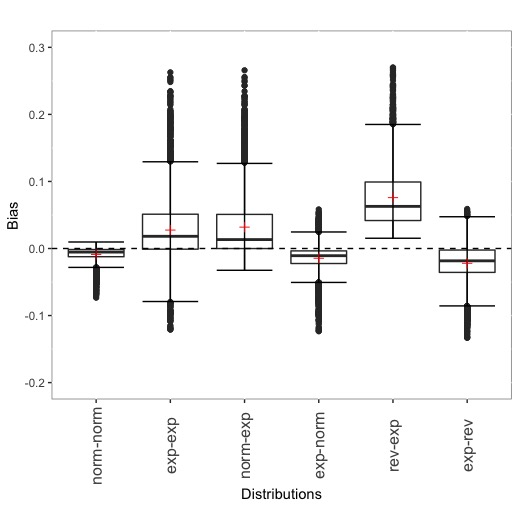
\includegraphics[width=\linewidth]{fig/bias_boxplot}
	\caption[Example of Figures.]{Example of figures. If the figure title is too long, you could the shortened title in the content. }
	\label{fig:ex1}
\end{figure}

%----------------------------Appendices----------------------------%
\newpage
\doublespacing
\appendix


\addappheadtotoc
\appendixtitleon
\appendixpage
\section{R codes}
\label{app:Rfleish}
How to have R codes: 
For example, I want to use the function \proglang{describeBy} in the package \proglang{psych} to compute: 
\begin{lstlisting}
describeBy(data, by = groups)
\end{lstlisting}
%\begin{appendices}

\end{document}